\section{Installazione sync engine}

\subsection{Installazione}
Per installare ed avviare il sync engine è necessario:
\begin{itemize}
	\item Scaricare tutto il contenuto della seguente Repository:
	
\centerline{\url{https://github.com/MercurySeven/project-SSD}}

	\item Estrarre il contenuto del file .zip ottenuto in una cartella a piacimento che sia al di fuori della cartella che si vuole sincronizzare;
	
\item Impostare PYTHONPATH:

Per impostare il PYTHONPATH bisogna utilizzare la keyword set su windows e la keyword export su macOS e Linux. La variabile bisogna impostarla al path assoluto dove si è estratto l'archivio.
Di seguito sono riportati due esempi, rispettivamente per windows e linux/macOS
\begin{figure}[H]
    \centering
    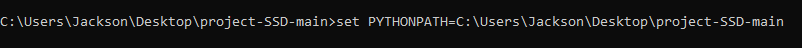
\includegraphics[scale = 0.65]{components/img/Windows-istruzione-1.png}
    \caption{Comando per impostare PYTHONPATH su windows}
    \label{fig:comando per impostare PYTHONPATH su windows}
\end{figure}
\begin{figure}[H]
    \centering
    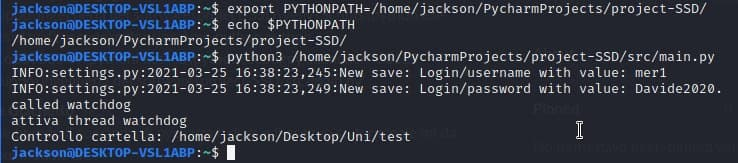
\includegraphics[scale = 0.65]{components/img/linux-istruzione-1.jpg}
    \caption{ Comando per impostare PYTHONPATH su linux}
    \label{fig:comando per impostare PYTHONPATH su windows}
\end{figure}

\item Avviare il programma utilizzando il comando python3 seguito dal path assoluto del file main.py. Di seguito viene riportato un esempio.
\begin{figure}[H]
    \centering
    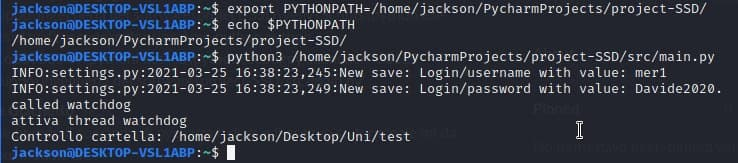
\includegraphics[scale = 0.65]{components/img/linux-istruzione-1.jpg}
    \caption{ Comando per avviare SSD}
    \label{fig:comando per impostare PYTHONPATH su windows}
\end{figure}

\end{itemize}